%%*****************************************************************************%%
%																				%
%																				%
%								LEAVE ME HERE									%
%																				%
%																				%
%              _____ ______   ________                   _______   				%  
%             |\   _ \  _   \|\   __  \                 /  ___  \    			%
%             \ \  \\\__\ \  \ \  \|\  \  ____________ /__/|_/  /|   			%
%              \ \  \\|__| \  \ \   _  _\|\____________\__|//  / /   			%
%               \ \  \    \ \  \ \  \\  \\|____________|   /  /_/__  			%
%                \ \__\    \ \__\ \__\\ _\                |\________\			%
%                 \|__|     \|__|\|__|\|__|                \|_______|			%
%                                                      							%
%																				%
%%*****************************************************************************%%
%									Links										%
%																				%
%		x Read only : https://www.overleaf.com/read/zpsfcpfhjdcc				%
%		x Edit&Read : https://www.overleaf.com/6786414fvkzzd					%
%		x Github	: https://www.github.com/MR-2								%
%																				%
%%*****************************************************************************%%
%							About - This Document								%
%																				%
%		x	 Analog Amplitude Modulation Plot Sample							%
%																				%
%		Note: Use it however you want.											%
%																				%
%%*****************************************************************************%%
%									Setup										%
%																				%

\documentclass[tikz,border=10pt]{standalone}
\begin{document}
    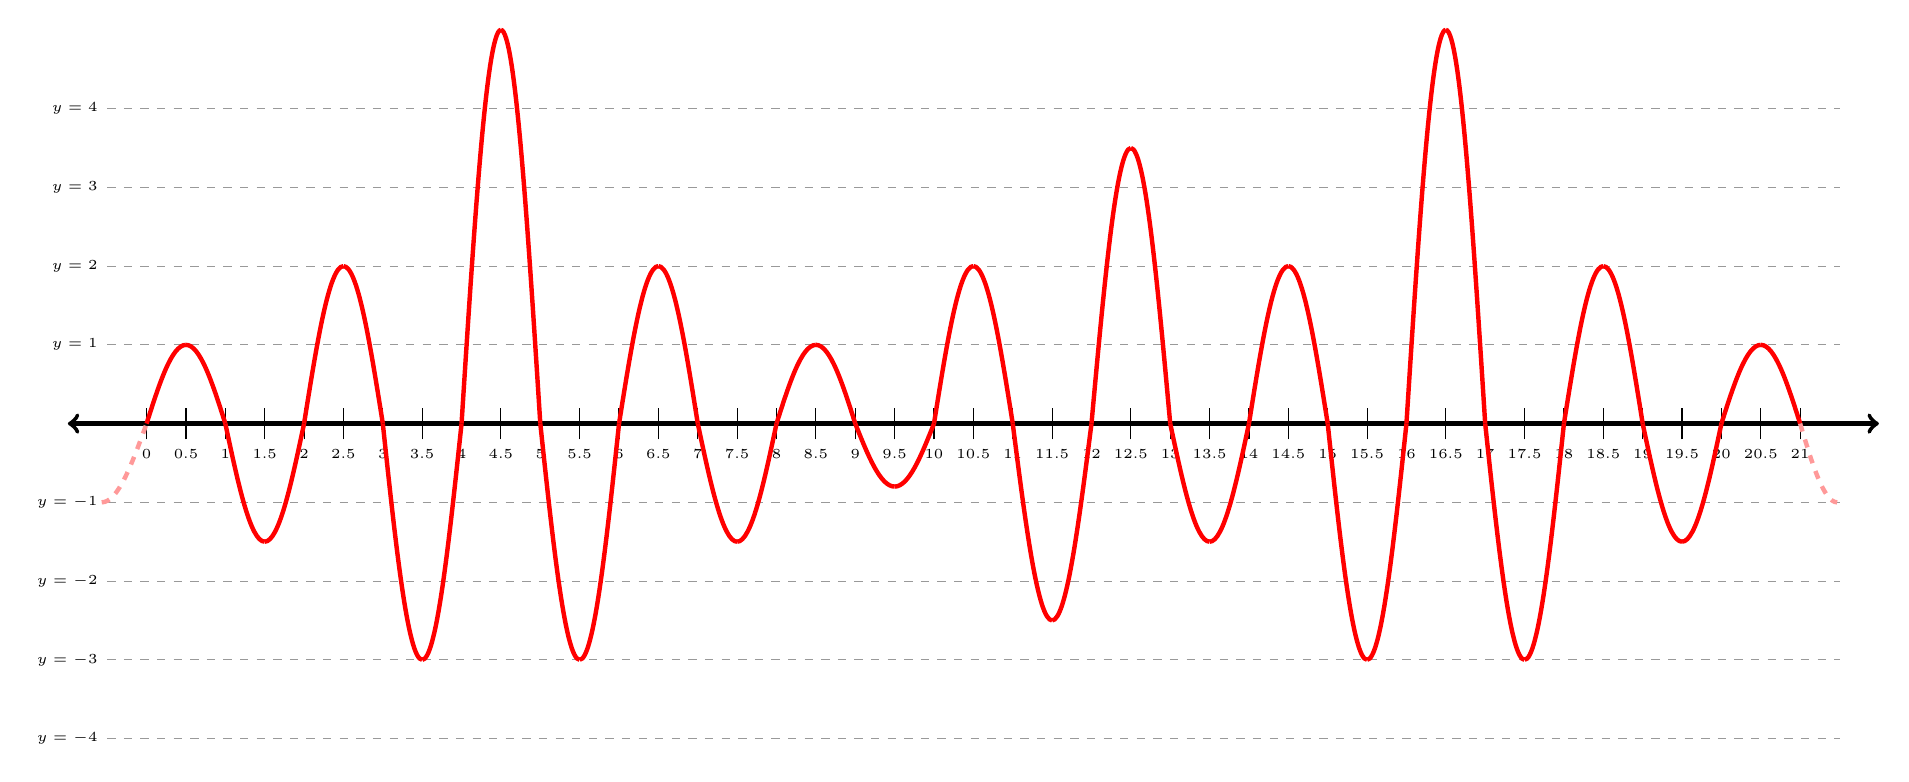
\begin{tikzpicture}
    \draw[ultra thick, black,<->] (-1,0) -- (22,0);
    \draw[dashed,draw=black!40] (-0.5,1)node[left,font=\tiny] {$y=1$} -- (21.5,1);
    \draw[dashed,draw=black!40] (-0.5,-1)node[left,font=\tiny] {$y=-1$} -- (21.5,-1); 
    \draw[dashed,draw=black!40] (-0.5,2)node[left,font=\tiny] {$y=2$} -- (21.5,2);
    \draw[dashed,draw=black!40] (-0.5,-2)node[left,font=\tiny] {$y=-2$} -- (21.5,-2); 
    \draw[dashed,draw=black!40] (-0.5,3)node[left,font=\tiny] {$y=3$} -- (21.5,3);
    \draw[dashed,draw=black!40] (-0.5,-3)node[left,font=\tiny] {$y=-3$} -- (21.5,-3);
    \draw[dashed,draw=black!40] (-0.5,4)node[left,font=\tiny] {$y=4$} -- (21.5,4);
    \draw[dashed,draw=black!40] (-0.5,-4)node[left,font=\tiny] {$y=-4$} -- (21.5,-4);
    \foreach \x in {0,0.5,...,21}{
    \draw (\x,-0.2)node [below,font=\tiny,] {\x} -- (\x,0.2) ;
    }
    
    
    \draw[ultra thick,dashed, red!40] (-0.57,-1) cos (0,0);
    \draw[ultra thick, red] (0,0) sin (0.5,1);
    \draw[ultra thick, red] (0.5,1) cos (1,0);
    \draw[ultra thick, red] (1,0) sin (1.5,-1.5);
    \draw[ultra thick, red] (1.5,-1.5) cos (2,0);
    \draw[ultra thick, red] (2,0) sin (2.5,2);
    \draw[ultra thick, red] (2.5,2) cos (3,0);
    \draw[ultra thick, red] (3,0) sin (3.5,-3);
    \draw[ultra thick, red] (3.5,-3) cos (4,0);
    \draw[ultra thick, red] (4,0) sin (4.5,5);
    \draw[ultra thick, red] (4.5,5) cos (5,0);
    \draw[ultra thick, red] (5,0) sin (5.5,-3);
    \draw[ultra thick, red] (5.5,-3) cos (6,0);
    \draw[ultra thick, red] (6,0) sin (6.5,2);
    \draw[ultra thick, red] (6.5,2) cos (7,0);
    \draw[ultra thick, red] (7,0) sin (7.5,-1.5);
    \draw[ultra thick, red] (7.5,-1.5) cos (8,0);
    \draw[ultra thick, red] (8,0) sin (8.5,1);
    \draw[ultra thick, red] (8.5,1) cos (9,0);
    
    
    \draw[ultra thick, red] (9,0) sin (9.5,-0.8);
    \draw[ultra thick, red] (9.5,-0.8) cos (10,0);
    \draw[ultra thick, red] (10,0) sin (10.5,2);
    \draw[ultra thick, red] (10.5,2) cos (11,0);
    \draw[ultra thick, red] (11,0) sin (11.5,-2.5);
    \draw[ultra thick, red] (11.5,-2.5) cos (12,0);
    \draw[ultra thick, red] (12,0) sin (12.5,3.5);
    \draw[ultra thick, red] (12.5,3.5) cos (13,0);
    
    
    \draw[ultra thick, red] (13,0) sin (13.5,-1.5);
    \draw[ultra thick, red] (13.5,-1.5) cos (14,0);
    \draw[ultra thick, red] (14,0) sin (14.5,2);
    \draw[ultra thick, red] (14.5,2) cos (15,0);
    \draw[ultra thick, red] (15,0) sin (15.5,-3);
    \draw[ultra thick, red] (15.5,-3) cos (16,0);
    \draw[ultra thick, red] (16,0) sin (16.5,5);
    \draw[ultra thick, red] (16.5,5) cos (17,0);
    \draw[ultra thick, red] (17,0) sin (17.5,-3);
    \draw[ultra thick, red] (17.5,-3) cos (18,0);
    \draw[ultra thick, red] (18,0) sin (18.5,2);
    \draw[ultra thick, red] (18.5,2) cos (19,0);
    \draw[ultra thick, red] (19,0) sin (19.5,-1.5);
    \draw[ultra thick, red] (19.5,-1.5) cos (20,0);
    \draw[ultra thick, red] (20,0) sin (20.5,1);
    \draw[ultra thick, red] (20.5,1) cos (21,0);
    
    \draw[ultra thick,dashed, red!40] (21,0) sin (21.47,-1);
    
    \end{tikzpicture}
\end{document}